\documentclass[11pt, oneside]{article}   	% use "amsart" instead of "article" for AMSLaTeX format
\usepackage[margin=1in]{geometry}                		% See geometry.pdf to learn the layout options. There are lots.
\geometry{a4paper}                   		% ... or a4paper or a5paper or ... 
%\geometry{landscape}                		% Activate for rotated page geometry
\usepackage[parfill]{parskip}    		% Activate to begin paragraphs with an empty line rather than an indent
\usepackage{graphicx}				% Use pdf, png, jpg, or eps§ with pdflatex; use eps in DVI mode
								% TeX will automatically convert eps --> pdf in pdflatex		
\usepackage{amsmath}
\usepackage{amssymb}
\usepackage{hyperref}          % hyperlink
\usepackage{color,soul}  % highlight
\usepackage{graphicx}    % include graphics

%SetFonts

%SetFonts


\title{Model}
\author{Lingjie}
%\date{}							% Activate to display a given date or no date

\begin{document}
\maketitle

\section{Stochastic discount factor (SDF)}

Arise from consumer maximising present and future utility by choosing asset amount

\begin{tabular}{l @{ := } l}
    $\xi$ & amount of asset \\
    $c_t$ & consumption at time $t$ \\
    $u(c_t)$ & utility at time $t$ \\
    $E_t(u)$ & expected utility at time $t$ \\
    $\beta$ & subjective discount factor \\
    $e_t$ & original consumption level at time $t$ \\
    $p_t$ & price of asset at time $t$ \\
    $x_t$ & payoff of asset at time $t$
\end{tabular}

\begin{align*}
    \max_{\xi} & ~u(c_t) + E_t\left[ \beta u(c_{t+1}) \right]~s.t.\\
    c_t &= e_t - p_t\xi \\
    c_{t+1} &= e_{t+1} + x_{t+1}\xi
\end{align*}

Solving for First Order Condition to find maxima

\begin{align*}
    p_tu'(c_t) &= E_t\left[ \beta u'(c_{t+1}) x_{t+1}  \right]\\
    \Rightarrow p_t &= E_t\left[ \beta \frac{u'(c_{t+1})}{u'(c_t)} x_{t+1}  \right] \\
    \Leftrightarrow p_t &= E_t \left[ m_{t+1} x_{t+1}  \right]
\end{align*}

where $m_{t+1}:=\beta\frac{u'(c_{t+1)}}{u'(c_t)}$ is defined as SDF

\section{No-Arbitrage Asset Pricing}

\subsection{No-arbitrage}

$m > 0 \Rightarrow$ No-arbitrage. Since marginal utility is assumed to be positive, $m > 0$.

No-arbitrage assumption $\Leftrightarrow$ there exist a $m_{t+1}$ such that

\begin{tabular}{l @{ := } l}
    $R^e_{t,i}$ & excess return of asset $i$ at time $t$ \\
    $R_{t,i}$ & actual return of asset $i$ at time $t$ \\
    $R^f_t$ & return of a risk free asset at time $t$
\end{tabular}

\begin{align*}
    R^e_{t+1, i} &= R_{t+1, i} - R^f_{t+1} = 0
\end{align*}

\subsection{exposure to systematic risk $\beta_{t, i}$ formulation}

Let $p_t = 0, x_{t+1} = R^e_{t+1, i} = 0 \Rightarrow E_t\left[ m_{t+1}R^e_{t+1, i}  \right] =0$

and
\begin{align*}
    E_t\left[ m_{t+1}R^e_{t+1, i}  \right] = 0 \Leftrightarrow E_t\left[ R^e_{t+1,i}  \right] 
    &= \left( - \frac{Cov_t(R^e_{t+1, i}, m_{t+1} )}{Var_t(m_{t+1})}  \right) \cdot \frac{Var_t(m_{t+1})}{E_t\left[ m_{t+1}  \right]} \\
    &= \beta_{t,i}\lambda_t
\end{align*}

to show $E_t\left[ R^e_{t+1, i}  \right] = \beta_{t, i}\lambda_t$

\begin{align*}
    E_t\left[ R^e_{t+1,i}  \right] &=
    \left( - \frac{Cov_t(R^e_{t+1, i}, m_{t+1} )}{Var_t(m_{t+1})}  \right) \cdot \frac{Var_t(m_{t+1})}{E_t\left[ m_{t+1}
    \right]} \\
                                   &= - \frac{Cov_t(R^e_{t+1, i}, m_{t+1})}{E_t\left[ m_{t+1}  \right]} \\
                                   &= - \frac{E_t\left[ R^e_{t+1, i}, m_{t+1}  \right] - E_t\left[ R^e_{t+1, i}
                                   \right]E_t\left[ m_{t+1}  \right]}{E_t\left[ m_{t+1}  \right]} \\
    \because E_t\left[ R^e_{t+1, i}, m_{t+1}  \right] &= 0 \\
    \Rightarrow E_t\left[ R^e_{t+1, i}  \right] &= E_t \left[ R^e_{t+1, i}  \right]~(shown)
\end{align*}

As shown, $E_t\left[ R^e_{t+1, i}  \right] = \beta_{t, i}\lambda_t$.

\begin{tabular}{l @{ := } l}
    $\beta_{t,i}$ & exposure to systematic risk \\
    $\lambda_t$ & price of risk \\
    $E_t[.]$  & expectation conditional on the information at time $t$
\end{tabular}

\subsection{SDF weight $\boldmath{\omega_t}$ and tangency portfolio $F_{t+1}$ formulation}

We will use

\begin{tabular}{l @{ := } l}
    $R^e_t$ & the vector representing $R^e_{t, i}$ for $i\in[1, N]$\\
    $\omega_t$ & the vector representing SDF weight $\omega_{t, i}$ for $i\in[1, N]$ \\
    $f_{t+1}$ & tangency portfolio, a scalar
\end{tabular}

Note $m_{t+1}$ is a scalar.

Now, since SDF is an affine transformation of the tangency portfolio ($m_{t+1} = a + b{f_{t+1}}$), we consider the
special case when $a=1, b=-1$, then

\begin{align*}
    m_{t+1} = 1 - f_{t+1} = 1 - \sum_{i=1}^N \omega_{t, i} R^e_{t+1, i} = 1 - {\omega_t}^T {R^e_{t+1}}
\end{align*}

where $f_{t+1} = \omega_t^TR^e_{t+1}$, the tangency portfolio is the weighted sum of excess returns.

\subsection{linking systematic risk $\beta_{t,i}$ to tangency portfolio $f_{t+1}$}

Now, since $m_{t+1} = 1 - f_{t+1}$, using previous result of 
\begin{align*}
    E_t[R^e_{t+1, i}] &= \left( - \frac{Cov_t(R^e_{t+1, i}, m_{t+1})}{Var_t(m_{t+1})}  \right) \cdot
    \frac{Var_t(m_{t+1})}{E_t[m_{t+1}]} \\
                      &= \left( - \frac{Cov_t(R^e_{t+1, i},(1-f_{t+1}))}{Var_t(1-f_{t+1})} \right) \cdot 
                      \frac{Var_t(1-f_{t+1})}{E_t[1-f_{t+1}]} \\
                      &= \frac{Cov_t(R^e_{t+1, i}, f_{t+1})}{Var_t(f_{t+1})} \cdot \frac{Var_t(f_{t+1})}{1 -
                      E_t[f_{t+1}]} \\
                      &= missing \\
                      &= \beta_{t, i} E_t[f_{t+1}]
\end{align*}

\hl{missing proving}

and $R^e_{t+1, i} = \beta_{t+1, i}\cdot f_{t+1} + \epsilon_{t+1, i}$

\section{Applying Generative adversarial network to estimate SDF}

There are two functions we are interested in finding:

\begin{enumerate}
    \item $\omega_t=\omega(I_t, I_{t, i})$
    \item $\beta_{t, i}=\beta(I_t, I_{t, i})$
\end{enumerate}

These two functions are sufficient for:

\begin{enumerate}
    \item Explain cross-section of individual stock return $R^e_{t+1, i}$
    \item Construct conditional mean-variance efficient tagency portfolio $f_{t+1}(\omega_t)$
    \item Decompose stock returns into their predictable systematic componenet $\beta_{t, i}, f_{t+1}$ and their non-systematic unpredictable
        component $\epsilon_{t+1, i}$
\end{enumerate}

We will be using GAN (Generative adversarial network) methods to deduce $\omega_t$, which will construct $f_{t+1}$ and 
later will be used to deduce $\beta_{t, i}$.

\subsection{Generative adversarial Methods of Moments}

GAN model requires 'Generator' and 'Discriminator'.

A generator predict the
outcome we are interested in (in our case, the function $\omega_t$) while a discriminator produces fake
data that meant to confuse the generator (a pricing error function $g$ which we will define later). 

A loss function links the generator and discriminator, and training will continue until
neither generator nor discriminator can improve their performance further.

\subsubsection{Input Data}

We denote the input data with:

\begin{tabular}{l @{ := } l}
    $I_t$ & macroeconomic data at time $t$, such as inflation\\
    $I_{t, i}$ & firm specific data at time $t$, such as book to market ratio
\end{tabular}

\subsubsection{Include macro economic features with RNN and LSTM}

Recurrent neural network (RNN) is a class of neural network that considers the past data in future prediction.

Long Term Short Term Memory (LSTM) is a subclass of RNN that considers dynamic past data in future prediciton.

LSTM is an improvement over vanilla RNN.
In a vanilla RNN, an unique weight is given to each of the lagged data. 
The number of lagged data will be pre-determined and could not scale well with higher lags.

LSTM solves the problem by introducing forget gate, input gate and output gate.
Simplify saying, LSTM endogenously handle the number of lags that will be useful in the prediction.

Since we suspect past macro economic feature will affect our estimation and we are uncertain how many lag terms
to include, we use RNN with LSTM to let the model decide the number lag terms.

\subsubsection{Generator: $\omega(I_t, I_{t, i})$}

Given that $f_{t+1}=\omega_t^T R^e_{t+1}$, we need $\omega_t$ and $R^e_{t+1}$

$R^e_{t+1}$ can be calculated with $R_{t+1} - R^f_{t+1}$ using price data.

Only estimation required will be $\omega(I_t, I_{t, i})$.

\subsubsection{Discriminator: $g(I_t, I_{t, i})$}

Under no arbitrage model, there exist a $m_{t+1}$ such that $E(m_{t+1}R^e_{t+1})=0$.

In a more general case, we can always find a uncondtional expectation where 

\begin{align*}
    E(m_{t+1}R^e_{t+1, i}g(I_t, I_{t, i}))=0
\end{align*}

$g$ represents factors unexplained by the no-arbitrage model, or a pricing error.

We will use $g$ as our discriminator.

\subsubsection{Loss function}

We can summarise the relationship between generator and discriminator using a 
min max optimization problem as the loss function.

We want to maximise the loss by changing function $g$ while minimise the loss by changing function $\omega$

\begin{align*}
    \min_{\omega} \max_{g} \frac{1}{N} \sum_{j=1}^N \left\{
    E \left[ 
        \left( 1 - \sum_{i=1}^N \omega(I_t, I_{t, i}) R^e_{t+1, i} \right)
        R^e_{t+1, j}g(I_t, I_{t, j})
    \right] \right\}^2
\end{align*}

the final estimated generator function $\hat\omega$ is

\begin{align*}
    \hat\omega &= \min_{\omega} L(\omega|\hat{g}, I_t, I_{t, i})
\end{align*}

which is the $\omega$ that minimise the loss function, with a given discriminator $g$.

\subsubsection{Model training and architecture}

GAN has a two step training procedure.

\begin{enumerate}
    \item Train $\omega$ while keeping $g$ unchanged
        \subitem $\min_{\omega} L(\omega|\hat{g}, I_t, I_{t,i})$
    \item Train $g$ while keeping $\omega$ unchanged
        \subitem $\max_{g} L(g|\hat\omega, I_t, I_{t,i})$
\end{enumerate}

The training will continue until neither $g$ nor
$\omega$ can reduce the loss further.

Both $g$ and $\omega$ will have the similar model structure.
However, $\omega$ will be used to construct $f_{t+1}$ while $g$ will be in its raw form.

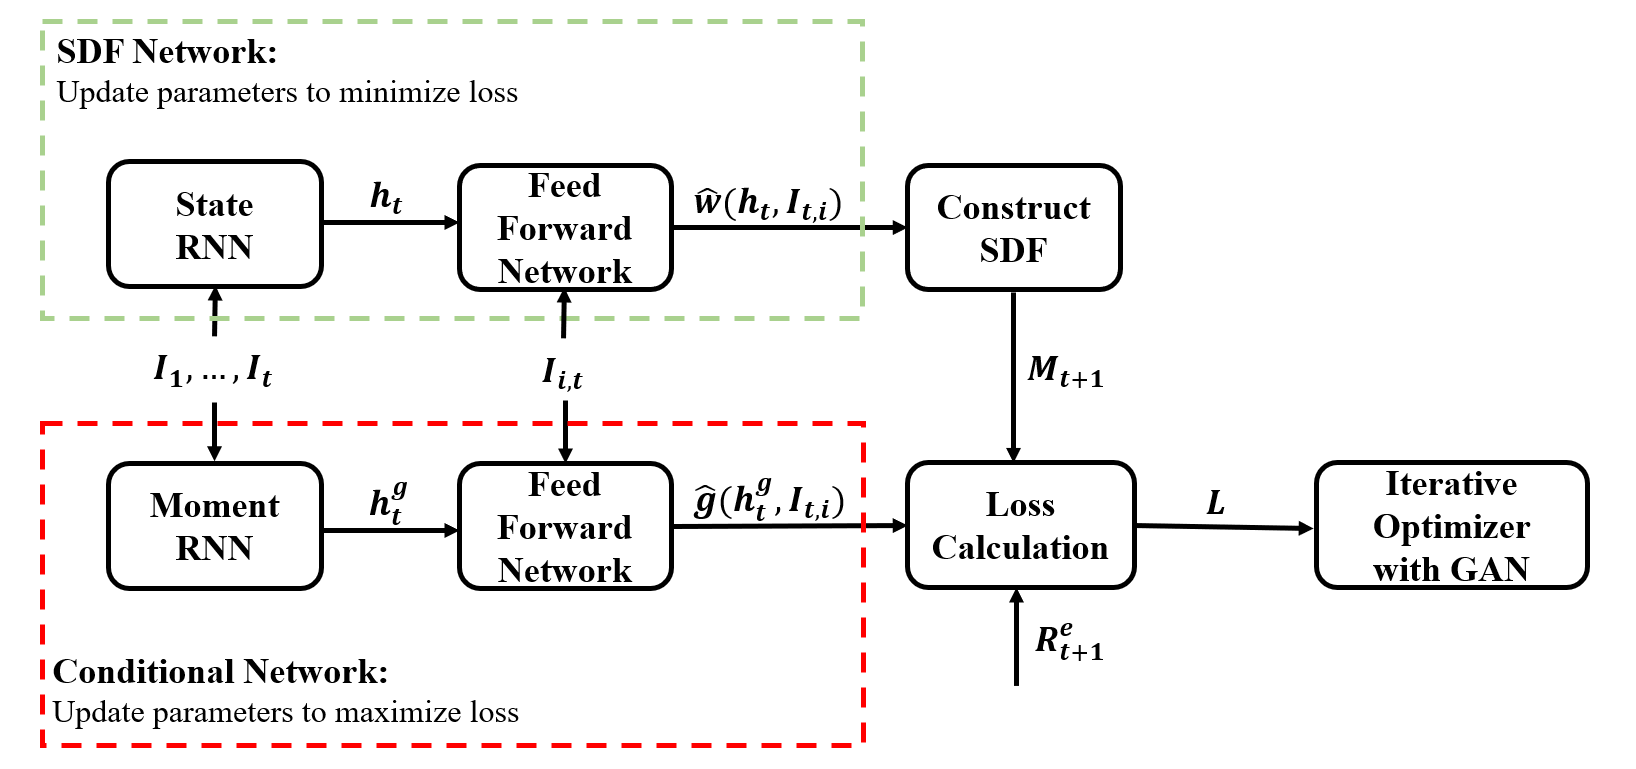
\includegraphics[width=\textwidth]{./reference_paper/img/model}

\end{document}
